% !TeX root = text.tex
\chapter{Software}

Tato kapitola se~zabývá softwarovou výbavou laserového projektoru. Popisuje klíčové programy, jejich funkce a~způsob, jakým mezi sebou komunikují.
Mezi tyto programy patří program lasershow, který obsluhuje vykreslování, programy pro~interakci s~uživatelem (dále \uv{frontendové programy}) jako UI, web\_ui a~discord\_bot, a~také program wifi\_manager, který spravuje wifi připojení Raspberry Pi.
Programy wifi\_manager a~lasershow se~dají označit za~backendové programy, protože neinteragují s~uživatelem.

V neposlední řadě popisuje také instalační skript, který výrazně zjednodušuje instalaci všech zmíněných programů a~jejich závislostí.

Program lasershow umí číst projekční soubory ve~formátu .ild.
Uživatel může takový soubor vytvořit například v~softwaru Laserworld Showeditor V7~\cite{showeditor} nebo může do~frontendových programů nahrát soubor v~populárním vektorovém formátu .svg a~frontendové programy využijí skript svg2ild.py dostupný~z~\cite{svg2ild}.

% O~řízení galvanometrů se~stará program lasershow, který je~psaný v~jazyce C++ pro~maximální rychlost. Tento program běží na~pozadí a~čeká na~příkazy od~programů určených k~interakci s~uživatelem. Na~tento program se~zaměřuje kapitola lasershow. \fxnote{TODO: odkaz}

% Dále jsou tu~programy, které se~starají o~interakci s~uživatelem. Tyto programy přijímají příkazy od~uživatele a~posílají je~programu lasershow. Navíc od~lasershow získávají výstup, který následně zprostředkovávají uživateli; důkladněji popsáno v~kapitole~\ref{sec:comms}.
% Mezi tyto programy patří programy UI, web\_ui a~discord\_bot. Program UI~spravuje OLED displej, přijímá od~uživatele vstup rotačním enkodérem a~je~psaný v~C++ pro~jednodušší interakci s~hardwarem. Program web\_ui využívá runtime Node.js, ve~kterém je~nenáročné vytvořit http server dostupný z~lokální sítě. \fxnote{(A)?} Program discord\_bot, také využívající Node.js, přijímá příkazy z~chatovací aplikace discord a~je~přístupný i~přes internet.

% Nakonec je~tu~program wifi\_manager, ten~spravuje wifi připojení RPi, je~psaný v~Node.js a~komunikuje s~programy, které interagují s~uživatelem stejně jako program lasershow.

\section{komunikace mezi programy}\label{sec:comms}
Všechny tyto programy jsou propojeny síťovými sockety zprostředkovanými knihovnou ZeroMQ, která nabízí frontu\footnote{Ve frontě jsou zprávy seřazeny od~té nejdříve odeslané.} zpráv, bez potřeby samostatně běžícího brokeru.

Tato knihovna je~využita k~vytvoření dvou socketů, jedním lasershow přijímá příkazy od~uživatele prostřednictvím ostatních programů (vstupní socket na~portu 5557, viz obr.~\ref{fig:tcp5557}) a~do~druhého posílá informace ostatním programům (výstupní socket na~portu 5556, viz obr.~\ref{fig:tcp5556}), aby je~zprostředkovaly uživateli.
Do~prvního zmíněného posílají progamy interagující s~uživatelem příkazy pro programy lasershow a~wifi\_manager. Do~druhého posílá lasershow informace o~stavu a~změnách nastavení  a~také wifi\_manager informace o~stavu a~změnách v~nastavení WiFi.

Příkazy pro programy lasershow a~wifi\_manager vypadají následovně
\fxnote{TODO: příklady příkazů pro lasershow a~wifi\_manager z~\url{https://github.com/phuid/laser_projector/blob/master/README.md}}
\fxnote{TODO: příklady status infos od~lasershow a~wifi\_manager z~\url{https://github.com/phuid/laser_projector/blob/master/README.md}}

\begin{figure}[htb]
  \centering
  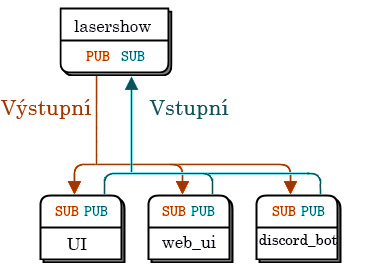
\includegraphics[width=0.5\textwidth]{img/comms_lasershow_scheme.jpg}
  \caption{\label{fig:lasershow_comms} Komunikace mezi programy vstupním socketem na~portu 5557}
\end{figure}
\begin{figure}[htb]
  \centering
  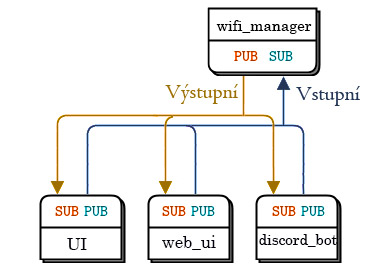
\includegraphics[width=0.5\textwidth]{img/comms_wifiman_scheme.jpg}
  \caption{\label{fig:wifiman_comms} Komunikace mezi programy výstupním socketem na~portu 5556}
\end{figure}

\section{lasershow}

Program lasershow je~psaný v~jazyce c++, který je~kompilovaný a~obecně považovaný za~jeden z~nejrychlejších jazyků. Druhé zmíněné se~hodí, jelikož chceme vykreslovat co~možná nejrychleji.

Tento program zaregistruje vstupní TCP socket na~portu 5557 a~knihovnou ZeroMQ se~na něm přihlásí k~odběru zpráv, které do~něj publikují ostatní programy. Zárověn podobně zaregistruje výstupní socket na~portu 5556, do~kterého později bude posílat zprávy pro programy, které interagují s~uživatelem.

Následně se~připojí k~DAC a~čeká na~zprávy od~ostatních programů. Jakmile zprávu obdrží, zpracuje ji~a pokud je~požadována změna nastavení, okamžitě ji~provede a~aktuální nastavení si~uloží do~souboru, jestliže je~požadováno vykreslení obrazu ze~souboru, začne obraz vykreslovat. Při tom průběžně posílá informace o~stavu vykreslování do~výstupního socketu. I~při vykreslování obrazu tento program zpracovává zprávy a~pokyny ze~vstupního socketu.

Program byl původně převzat z~projektu \url{https://github.com/tteskac/rpi-lasershow}\footnote{staženo 28.~12.~2023}, následně byl ale přepsán skoro ve~všech ohledech a~z původního programu zbylo asi 20 řádků.
\fxnote{TODO: odkud jsem to~vzal a~prepsal a~jak moc jsem toho udelal a~s jakymy vysledky}

\fxnote{TODO: diagram programu}

\fxnote{TODO: priklad zmq}\

\fxnote{ use \url{https://cs.overleaf.com/learn/latex/Code_Highlighting_with_minted} instead - function highlights}

\lstinputlisting[language=c++, style=code]{code_examples/zmq_server.cpp}
\lstinputlisting[language=c++, style=code]{code_examples/zmq_client.cpp}


\section{wifi\_manager}

V rámci této práce byl vyvinut ještě jeden program, který se~přímo nepodílí ani na~projekci, ani na~interakci s~uživatelem.

Program wifi\_manager je~také napsaný v~jazyce JavaScript s~využitím runtime Node.js. Registruje se~ke stejným socketům jako lasershow, přijímá příkazy týkající se~nastavení WiFi na~Raspberry Pi~TCP socketem na~portu 5557 a~odesílá zpětnou vazbu na~TCP socket s~portem 5556.

\fxnote{TODO: jak se~komunikace s~lasershow odlisuje od~wifi\_managera}

\fxnote{TODO: ukazka(idk what)}

Hlavním úkolem tohoto programu je~správa a~konfigurace WiFi připojení na~Raspberry Pi. Přijímá příkazy od~ostatních programů a~nastavuje WiFi parametry na~základě těchto příkazů. Tím umožňuje uživatelům snadno a~pohodlně nastavit WiFi připojení na~svém zařízení.

Stejně jako lasershow, wifi\_manager také posílá zpětnou vazbu ostatním programům, aby informoval o~stavu a~změnách v~nastavení WiFi. Tímto způsobem je~zajištěna komunikace a~synchronizace mezi všemi programy v~laserovém projektoru.

Celkově wifi\_manager přispívá k~plynulému a~efektivnímu provozu laserového projektoru tím, že umožňuje snadnou správu a~konfiguraci WiFi připojení na~Raspberry Pi.

\section{UI}
Program UI~je~také psaný v~jazyce c++ a~. Tento program ovládá OLED displej, který je~připojený na~Raspberry Pi~pomocí rozhraní I2C, a~přijímá vstup od~uživatele čtením rotačního enkodéru s~tlačítkem. Také příjmá informace od programů lasershow a wifi\_manager a posílá jim vstup od uživatele.

Na LCD displeji má uživate ldíky tomuto programu přístup k menu, kde jsou zobrazeny aktuální informace o promítání a wifi připojení a kde uživatel může měnit nastavení dvou backendových programů.

\subsection{Využité knihovny}
\subsubsection{wPi\_soft\_lcd}
Hlavní využitou knihovnou je wPi\_soft\_lcd~\cite{wpi-lcd}. Tato knihovna umožňuje jednoduchou komunikaci s LCD prostřednictvím I$^{2}$C převodníku. 

Mezi nejdůležitější funkce této knihovny, které používám ve svém kódu patří:
\begin{itemize}
  \item \mintinline{cpp}{lcd_t *lcd_create(int scl, int sda, int addr, int lines)} --- Tato funkce inicializuje komunikaci s I$^{2}$C převodníkem. Je nutné ji zavolat před jiným použitím knihovny. Příjmá čísla pinů I$^{2}$C sběrnice, na které je připojený displej, dále příjmá I$^{2}$C adresu převodníku a počet řádků displeje. Funkce vrací pointer na nově vytvořenou strukturu typu \mintinline{cpp}{lcd_t}, který je potřeba k volání dalších funkcí knihovny. Jestliže se nepodaří inicializovat knihovnu, vrací hodnotu \mintinline{cpp}{NULL}.
  \item \mintinline{cpp}{void lcd_printf(lcd_t *lcd, const char* format, ... )} --- K vypsání textu na LCD využívám tuto funkci. Příjmá pointer vrácený funkcí \mintinline{cpp}{lcd_create}, formátovací řetězec a případně další argumenty stejně, jako známá funkce \mintinline{cpp}{printf} ze standartní knihovny programovacího jazyka C.
  \item \mintinline{cpp}{void lcd_clear (lcd_t *lcd)} --- Funkce při jejím zavolání vymaže všechen text zobrazený na LCD. Příjmá pointer funkcí \mintinline{cpp}{lcd_create}.
  \item \mintinline{cpp}{void lcd_pos(lcd_t *lcd, int row, int col)} --- Touto funkcí je možno nastavit pozici virtuálního kurzoru, od kterého začne vypisovat funkce \mintinline{cpp}{lcd_printf}. Příjmá  pointer funkcí \mintinline{cpp}{lcd_create}, číslo řádku a číslo sloupce požadované pozice kurzoru. Obě čísla jsou počítaná od nuly.
  \item \mintinline{cpp}{void lcd_backlight_dim (lcd_t *lcd, float intensity)} --- Funkce, která nastaví střídu PWM signálu na GPIO pinu 18 a tím reguluje jas podsvícení LCD. Příjmá pointed vrácený funkcí \mintinline{cpp}{lcd_create} a desetinné číslo od 0 do 1, značící požadovanou intenzitu podsvícení.
  \item \mintinline{cpp}{void lcd_create_char(lcd_t *lcd, int n, char *data)} --- Touto funkcí je možné definovat vlastní znaky, které se zobrazí na LCD. Příjmá pointer vrácený funkcí \mintinline{cpp}{lcd_create}, číslo znaku, který má být definován a pole 8 bytů, které reprezentuje vlastní znak.
  \item \mintinline{cpp}{}
  \item \mintinline{cpp}{}
  \item \mintinline{cpp}{}
  \item \mintinline{cpp}{}
\end{itemize}

\subsubsection{wiringPi}
Předchozí popsaná knihovna pro posílání signálu I$^{2}$C sběrnicí používá knihovnu wiringPi, která umožňuje ovládání GPIO pinů. Abych nepřidával do jednoho programu dvě knihovny interagující s hardwarem, stejnou knihovnu využívám pro čtení dat z enkodéru.

Je nepraktické využívat v tomto programu jinou knihovnu na interakci s hardwarem, proto v budoucnu přepíši knihovnu wPi\_soft\_lcd tak, aby i ona využívala modernější knihovnu pigpio popsanou v kapitole \ref{sec:ls_pigpio}.

\begin{itemize}
\item \mintinline{cpp}{void pinMode (int pin, int mode)} --- Funkce, která pro GPIO pin z argumentu \mintinline{cpp}{pin} nastaví mód z argumentu \mintinline{cpp}{mode}. Jako argument \mintinline{cpp}{mode} používám hodnotu \mintinline{cpp}{INPUT}, která pin zaregistruje pro vstup.
\item \mintinline{cpp}{void pullUpDnControl (int pin, int pud)} Funkce připojí na pin \mintinline{cpp}{pin} pull-up nebo pull-down rezistor podle argumentu \mintinline{cpp}{pud}. Jako argument \mintinline{cpp}{pud} používám hodnotu \mintinline{cpp}{PUD_UP}, která k pinu připojí pull-up rezistor.
\item \mintinline{cpp}{int wiringPiISR (int pin, int mode, void (*function)(void))} --- Tato funkce nastaví přerušení na pin \mintinline{cpp}{pin}. Tak, aby při změně hodnoty na tomto pinu byla zavolána tzv. callback funkce z argumentu \mintinline{cpp}{function}. Argument \mintinline{cpp}{mode} úrčuje, jestli je funkce zavolána pouze při tzv. rising edge, tzv. falling edge, nebo při obou. Já v tomto argumentu používám hodnotu \mintinline{cpp}{INT_EDGE_BOTH}.
\end{itemize}

\subsubsection{cppzmq}
Samozřejmě program také využívá knihovnu cppzmq dostupnou z \cite{cppzmq} a popsanou v kapitole \ref{sec:ls_cppzmq}. Program ji používá podobně jako program lasershow, ne však stejně.

Největším rozdílem je, že místo funkce \mintinline{cpp}{void zmq::socket_t::bind} používá funkci \mintinline{cpp}{void zmq::socket_t::connect(const char *addr_)}.
Funkci bind je totiž potřeba zavolat přesně jednou pro každý socket.
Jestliže ji už pro sockety zavolal program lasershow a socket tedy už je registrovaný k danému portu, je třeba zavolat funkci \mintinline{cpp}{connect}.

Dále samozřejmě stejně jako všechny frontendové programy do vstupního socketu zprávy posílá a z výstupního socketu zprávy čte.

\subsection{Struktura programu}
Program začne inicializací komunikace s LCD.
Poté pokračuje registrací interruptů na pinech, ke kterým je připojen enkodér. A následně se připojí k socketům aplikací lasershow a wifi\_manager.

V další části programu je definováno samotné menu. To má podobu struktury \mintinline{cpp}{menu_option}, která je definována následovně.

\begin{minted}{cpp}
struct menu_option
{
  std::string name;

  std::string command_name;

  menu_option_style style = UNDEFINED;

  std::vector<menu_option> nested_menu_options = {};
  uint8_t nest_selected = 0;
  uint8_t nest_scroll = 0;
  bool nest_option_active = 0;
  bool redraw = 0;

  menu_val<float> value;

  bool has_function = 0;
  void (*function)(zmq::socket_t &, menu_option &);
};
\end{minted}

Díky ní může definice menu vypadat například takto:

\begin{minted}{cpp}
  menu_option root = {
        .name = "ROOT",
        .style = ROOT_MENU,
        .nested_menu_options = {
            {
                .name = "progress%",
                .command_name = "progress",
                .style = VALUE,
                .value = {0, 0, 100, 0.5},
            },
            {
                .name = "current_frame",
                .command_name = "current_frame",
                .style = VALUE,
                .value = {1, 1, 1, 1},
            },
            {.name = "-no out received-",
             .style = TEXT},
            {.name = "STOP",
             .command_name = "STOP",
             .style = TEXT,
             .has_function = 1,
             .function = send_option_command},
            {.name = "PAUSE", .command_name = "PAUSE", .style = TEXT, .has_function = 1, .function = send_option_command},
            {
                .name = "PROJECT",
                .style = NESTED_MENU,
                .has_function = 1,
                .function = fill_with_files,
            },
            {
                .name = "options",
                .style = NESTED_MENU,
                .nested_menu_options = {
                    {
                        .name = "screen brightness",
                        .command_name = "screen_brightness",
                        .style = VALUE,
                        .value = {50, 0, 100},
                    },
                    {
                        .name = "repeat",
                        .command_name = "repeat",
                        .style = VALUE,
                        .value = {0, 0, 1, 1},
                    },
                    {
                        .name = "point_delay",
                        .command_name = "point_delay",
                        .style = VALUE,
                        .value = {0, 0, 10000, 10},
                    },
                    {
                        .name = "target_frame_time",
                        .command_name = "target_frame_time",
                        .style = VALUE,
                        .value = {0, 0, 10000, 1},
                    },
                    {
                        .name = "trapezoid_horizontal",
                        .command_name = "trapezoid_horizontal",
                        .style = VALUE,
                        .value = {0, -1.f, 1.f, 0.05},
                    },
                    {
                        .name = "trapezoid_vertical",
                        .command_name = "trapezoid_vertical",
                        .style = VALUE,
                        .value = {0, -1.f, 1.f, 0.05},
                    },
                },
                .has_function = 1,
                .function = read_options,
            }}};
\end{minted}

Následuje nekonečný cyklus, ve kterém program příjmá zprávy od programů lasershow a wifi\_manager a volá funkci menu\_interact, kter

\subsection{vysledekdsdsa}

\section{web\_ui}

Narozdíl od~předchozích dvou zmiňovaných programů je~program web\_ui psaný v~jazyce javascript, ten nepatří mezi nejrychlejší, ale díky runtime Node.js a~knihovnám http a~formidable v~něm bylo časově nenáročné vytořit http web server.

Tento server běží na~portu 3000 a~je~dostupný z~lokální sítě (tzn. přímo z\~Raspberry Pi~na~adrese http://localhost:3000 nebo z~jakéhokoliv zařízení na~stejné lokální síti na~ip~adrese RPi).
Program je~využíván pro jednoduchou interakci s~uživatelem, který může pomocí webového prohlížeče ovládat laserový projektor pár kliknutími i~zadávat vlastní příkazy klávesnicí.

\fxnote{na webu jsou konzole pro ssh, wifiman a~lasershow, taky fast project forms, queue, settings, a chtel jsem pridat i kamerove online ukozovatko}

\fxnote{TODO: příklad http serveru}
\inputminted{js}{code_examples/http_static_files.js}

Stejně jako program UI~za~pomoci knihovny ZeroMQ tento program odebírá z~výstupního socketu zprávy o~průběhu vykreslování od~programu lasershow a~odesílá mu~pokyny uživatele na~vstupní socket.

\fxnote{TODO: příklad přihlášení k~socketům v~js}

\fxnote{TODO: xterm + ssh}

\section{discord bot}

Posledním programem, který je~využíván k~interakci s~uživatelem je~discord\_bot, který je~také psaný v~jazyce javascript v~runtime Node.js, stejně jako předchozí programy se~přihlásí k~socketům knihovnou zmq, ale na~rozdíl od~nich tento program může interagovat s~uživatelem přes internet ať už je~kdekoliv na~světě.
Pomocí knihovny discord.js se~přihlásí k~předem vytvořenému bot účtu, který může na~předem vytvořeném discord serveru čekat na~zprávy od~uživatele, ty~posílat do~vstupního socketu a~posílat uživateli zpětnou vazbu, kterou příjme z~výstupního socketu.



\section{Instalační skript}
Nedílnou součástí softwarové výbavy projektoru je~instalační skript.
Ten je~psaný v~příkazovém jazyce bash, který odpovídá sekvenci příkazů v~příkazovém řádku.
Instalační skript umožňuje instalaci celého projektu pouze třemi příkazy, viz~ukázka kódu~\ref{list:installcmds}.

\begin{code}
  \captionof{listing}{\label{list:installcmds} Příkazy potřebné k~instalaci projektu}
\begin{minted}[frame=lines,fontsize=\footnotesize,linenos]{shell}
  git clone https://github.com/phuid/laser_projector.git
  cd laser_projector
  bash install.sh
\end{minted}
\end{code}

Instalační skript stáhne a~nainstaluje nainstaluje veškeré závislosti a~knihovny ostatních programů. Stáhne také samotný interpreter Node.js.
Následně zkompiluje programy psané v~C++ a~nainstaluje a~nastaví služby potřebné k~vysílání hotspotu. Poté pomocí manažeru procesů pm2 dostupného z~\cite{pm2} nastaví automatické zapínání ostatních programů a~po~potvrzení uživatelem systém restartuje, aby~provedené změny nabyly efekt.
